\chapter{Conclusions}
\label{Chapter6}
\lhead{Chapter 6. \emph{Conclusions}}

\begin{figure}[H]
  \centering
  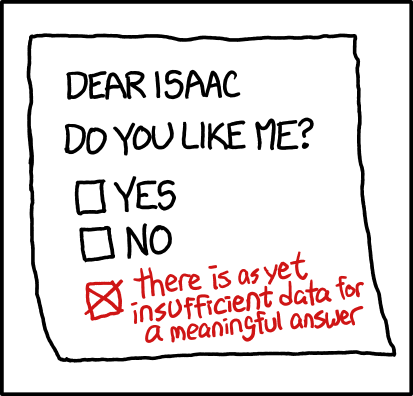
\includegraphics{Figures/xkcd/chapter6.png}
  \caption*{xkcd.com/1448}
\end{figure}

In this thesis I have aimed to demonstrate the ability to photometrically classifing SLSNe amongst large samples of transients detected by modern, wide-field astronomical surveys. In order to achieve this, I have combined our understanding of this class of objects with state-of-the-art Machine Learning and light curve modelling techniques to both define and predict their behaviour in a number of surveys. All this was performed with the aim of broadening our understanding of SLSNe as a population. The main results are summerised below.

\section{Modelling SN light curves}
In \cref{Chapter3}, I described the methods for modelling of CCSN and SLSN. I discussed both the analytical models as well as the the tools built to implement them. Furthermore, I described the Bayesian approach to the problem of model optimisation and introduces Gaussian Processes as a tool for non-parametric, probabilistic light curve interpolation.

\subsection{Modelling SLSNe}
The simulations of SLSNe at any redshift or bandpass were essential for this thesis. In \sref{sec:SLAP}, I demontrated an approach to producing a high quality SLSN SED model based on the black-body approximation of its continuum, combined with a spectral absorption template. The templates, focusing on the UV regions of the SED, significantly increased the redshift range at which I could confidently model these objects. I combined this with the evolution of the bolumetric luminosity of SLSNe based on the birth and spin-down of a magnetar model, modified to include a variable opasity term. I showed that this treatment of SLSNe correctly accounts for their light curve morphonogy including the late time evolution which is difficult to capture using other models.

\subsection{Modelling CCSN}
While CCSN are a better understood class of transients than SLSNe, their simulation tools are still lacking, specially in comparison to SN\,Ia. Here, I developed a set of tool for the modelling and simulations of CCSNe including both their hydrogen poor and rich subclasses. I provide a self contained solution, beginning with the archival photometry and spectroscopy for a number of nearby objects. Using an approach similar to \citet{Bazin2009}, I model their light curves in order to provide an interpolation model used to flux calibrate the observed spectra in the process refered to as mangling. Based on this approach, I built CoCo, a tool for generating spectral templates as well as using them to simulate these SNe.

The simulations work on a principle of placing the spectral template at any required redshift, then passing it through a bandpass filter, measuring the synthetic flux at the phases of the spetra, before fitting a light curve model to them to obtain flux at any arbitrary point in the light curve. Due to the wavelength limitations of ground based spectroscopy, the SED had to be extended in both IR and UV regimes. I used a combination of auxillary \textit{Swift}-UVOT data and the modelling of their continuum as dust extincted black-bodies to achieve a wavelength coverage down to $\sim1500\AA$, sufficient to measure the flux of a CCSN in the DES \textit{g}-band at their detection limit of z$\sim$0.7.

\subsection{Light Curve interpoaltion using Gaussian Processes}
Mate\'rn 3/2 kernel to model the covariance function of the data as I found it to be the best overall match to the typos of transients detected by DES.

\section{Rates of SLSN}
\cref{Chapter4} of this thesis focused on measuring the rate of SLSNe at the intermediate redshift of z$\sim$1. This was motivated by the low numbers of similar measurements, despite being a crucial piece of the puzzle of the origin on SLSNe. I provided one of the most accurate measurements of the rate, allowing us for the first time to probe the its evolution with redshift as well as the connection to other rare classes of transients.

\subsection{Defining SLSNe}
Starting from the SLSN models, based on the spin-down of a magnetar, I postulated a definition the SLSNe. After fitting the literature sample of these objects with the model, I found that SLSN concentrate in a small region of the P$_{ms}$-B$_{14}$-$\mathrm{\tau}_M$ parameter space, clearly separated from a majority of transients detected my the SNLS. I parametrised this region using an ellipsoid that tightly encapsules the entire training sample, giving a definition of a SLSN in terms of the parameter space of the magnetar model.

\subsection{Search for SLSN in SNLS}
I used my proposed definition of SLSNe to search for the presence of new, previosly unclassified SLSNe in the SNLS. Upon fittin its entire archival sample of transients, taking either their precise spectroscopic redshift (where available) or a range of host galaxy photometric redshift estimates I find that only two new objects fall within my definition. While one of the objects shows signs of multiseason variability, the second object, SNLS07D3bs, was found to be a strong SLSN candidate. My modelling suggested a good match to the class at 0.6$<$z$<1$. Using a low Sn\/N, archival spectrum of the object we were unable to confirm the classifcation, however, we used narrow line features to determine the true redshift of the object as z=0.74, confirming the object to be consistent with a luminosity of a SLSN.

\subsection{Rate of SLSNe at z$\sim$1}
With three SLSN candidates found in the SNLS, I performed a Monte Carlo simulation of the survey, replicating its transient detection behaviour. This reversed the common approach of calculating the rate of SNe by weighing each objects by its detection efficiency and observed volume. Instead, I simulated SLSNe before applying the survey noise and measuring each objects detectibility in the survey. Throughout the simulation, I iterate over a range of rate values to measure the resulting number of simualated detections. I then transpose these results to give me the probability of detecting 3 objects as a function of the input value. I found the rate of SLSNe at z$\sim$1 to be $91^{+76}_{-36}$\,SNe\,Yr$^{-1}$\,Gpc$^{-3}$ or 2.2$^{+1.8}_{-0.9}\times10^{-4}$ of the CCSN rate. This is consistent with similar pulications and tentitively demonstrates that the rate of SLSNe follows that of the star formation rate of the universe.

\subsection{Connection between SLSNe and ULGRBs}
An interesting question that we probed in \citet{Prajs2016} is the connection between the class of SLSNe and ULGRBs. LGRB are known to be connected to ordinary, stripped-envelope SNe as they result in the formation of a collapsar, or a jet forming young black hole powered by the infalling ejecta. Thanks to the advances in GRB observation provided by the \textit{Swift} satellite, we now know that some LGRB are observed to emmit $\gamma$-radiation for up to 10,000s. Classified as ULGRB, these events are known to be rarer than than ordinary LGRBs with their exact rate difficult to estimate due to the design of \textit{Swift}.

The discovery of an ULGRB, GRBXXXX introduced us to a potential connection to SLSNe as the object was observed as SN2011kl, an SN with a luminosity and monrphology similar to that of a number of lower luminosity SLSNe. It was also shown to have very similar spectroscopic characteristics.

\section{Photometic classification of SN}
Photometric classification of SNe forms the center piece of this thesis. Performed using a number of method, I demonstrate that the ML apprach is by far the most powerful approach to the problem, albeit, not the most straightforward to implement. While it required the construction of a large, artificial training sample, the results obtained using this method have largely exceeded the capabilities of other tools publically available to date.

\subsection{Training sample}
Using the combination of readily available models for SN\,Ia and AGNs as well as custom build models of SLSNe and CCSN, I have build a large training sample of transient light curves. I applied survey noise and cadance to match it properties with the real DES transient sample. The final sample consisted of $\sim$300,000 object, therefore being the largest, to date, light curve collection used for a photometric classification study and represents objects from low redshift, local objects to those that lay at the edge of DES detectibility.

\subsection{Machine Learning Model}
I developed a two stage approach to the problem of classifying DES transiants in order to reduce the number of free parameter in the model. In the first step, I separate SN (regardless of their class) from other contaminants in the sample, including AGNs and spurious noise detections. This focuses on long term variability of the object rather than the detailed evolution, used in the next stage to subdivide the SN sample
into their respective classes. This approach produces an excellent classification rate, correctly identifying 99.81\% SNe in the training sample. This was verified using a ground-truth sample where all spectroscipically confirmed transients (SNe and AGN) were correctly identified in this work.

Similarly to the SN identification pipeline, the SN classification algorithm has exceeded our expectations in terms of its accuracy. Compared to other similar projects, I did not use the spectroscopic redshift as a classification prior but, with a 97.85\% classification rate, I achieved a higher precision than reported by the current state-of-the-art solution \citep{Lochner2016}. Upon identifying the samlke of DES SNe, consiting of 5273 objects, I again tested the model against a ground-truth sample of spectroscopically confirmed SN\,Ia, correctly identifying 243 out of 250 objects. It is even more encouraging to mention that the misclassified objects formed extreme season edge cases where no data was observed near the maximum light for these objects.

Applying this technique to the full sample of DES transients, I identified 3120 potential SL\,Ia as well as 500 SLSN candidates. The later number vastly exceeded our expectations based on the rate of SLSNe measured in \cref{Chapter4}. The visual instection of the data showed that the sample is heavily contaminated by SN\,IIP, with characteristic long, red and platoeing light curves. We can attribute this to the lack of similar objects in the training sample as no objects of this class have passed the quality cuts required to generate a \textsc{CoCo} temaplete

\subsection{Selecting SLSN}
text

\section{Future Work}
Having developed a successful approach for the photometric classification of SLSNe in large astronimical surveys, there a number of avenues that I would like to pursue in the future. This includes both the improvement and application of the mothod to in future surveys as well as using the already extracted data to solve some of the yet to be explained misteries of SLSNe.

\subsection{Expanding the Training Sample}
One of the biggest issues identified in the process of photometrically classifing SLSNe was the incompleteness of the SN sample used in training of the ML algorithm. The lack of examples of SN\,IIP had the greatest effect as it introduces large number of inpurity in the sample of SLSNe. However the lack of other classes including rapidly evolving SNe and tidal disruption events also means that we cannot treat the samples of photometrically identified SN\,Ia and CCSNe as pure sample.

In this thesis, the training sample was based on the spectroscopic templates for each class geberated from the archival data for some of their most well observed examples. While the techniques have generally varied in details, they all required spectroscopic data to some extend. However, for a number of classes or rare and fast transients spectrscopy is very scarse while their photometries remain relatively abundant. A new approach, not requiring such extensive commitment from the data, is needed to extend the training samples. A possible solution, however requiring a large commitment of resources, would be to use physically motiated simuations to produce sample of objects and test their similarity to the available photometric samples. This approach is likely the most viable approach to the problem of modelling SN\,IIP where we could base the modelling on the existing simulations \citep{Dessart2013,Dessart2016}. 

\subsection{Rates of SLSNe from DES}
A natural extention of the work undergone in Chapters \ref{Chapter4} and \ref{Chapter5} is to compute the rate of SLSN using this new and expanded sample of objects. The improvement from 3 to XX objects alone will result in a vastly descred uncertainties in the overall rate of SLSNe. However, more importantly it will be the first ever measurement that will allow for a separation of the rate into separate reshift bins using a homogeneus sample.

\subsection{Properties of SLSNe}
text

\subsection{Selecting SLSN in LSST}
The upcoming decad

\subsection{Redshift estimation for photometric SN\,Ia in DES}
Perhaps one of the most interesting results in this thesis, not directly related to the main subject of SLSNe, is the accuracy of the photometric classification of SN\,Ia. This i slikely a reflection of the fact that the models for this class of SNe are mature with well understood parameter spaces producing a very
